\section{Task 1: Number Theory and Algebra}

\subsection{Explain why the integers Z form a ring, and the rationals Q form a field.}


A ring is a set R with two operations "+" and "*". (R,+) is an abelian group, that means it is associative, commutative and has a neutral and inverse element. (R,*) is a monoid, that means it is associative and has a neutral element. Lastly multiplication is distributive with respect to addition. If all axioms hold, a set is a ring. And they hold for Z.


A field is a ring but with the special case that $(R \backslash \{0\}, *)$ is an abelian group. Meaning that associativity and commutativity hold for all elements except 0 and that there also exists a neutral and inverse element for every element of the field.

\subsection{Find the inverses of all elements in Z\textsubscript{7}\textsuperscript{*}. Why do all numbers between 1 and 6 have an inverse?}

$Z^*_7 = {1,2,3,4,5,6}$\\
A number is an inverse, if number mod inverse = 1 (the neutral element)

\begin{tabular}{l c c c c c c}
	Number: & 1 & 2 & 3 & 4 & 5 & 6\\
	Inverse: & 1 & 4 & 5 & 2 & 3 & 6\\
\end{tabular}


If n is a prime, then all numbers between 1 and n-1 have an inverse with the modulo-Operation. This is due to n not being a multiple of any of the elements in the set.

\subsection{As an exercise, calculate the inverse of 331 in Z\textsubscript{1234} using the extended euclidean algorithm.}

GCD = 1, if Rest is 0 in the end\\
$1234  ==  3 * 331 + 241\\
331 == 1 * 241 + 90\\
241 == 2 * 90 + 61\\
90 == 1 * 61 + 29\\
61 == 2 * 29 + 3\\
29 == 9 *  3 + 2\\
3 ==  1 * 2 + 1\\
2 == 2 * 1 + 0$\\

Applying the algorithm:\\
$1 == 3 - 1 * 2\\
1 == 3 -  (29 - 9 * 3)\\
1 ==  10 * 3 - 1* 29\\
1 == 10 * (61 -  2 * 29) - 1 * 29\\
1 == 10 * 61 - 21 * 29\\
1 == 10 * 61 - 21 * (90 - 1 * 61)\\
1 == 31 * 61 - 21 * 90\\
1 == 31 * (241 - 2 * 90) - 21 * 90\\
1 == 31 * 241 - 83 * 90\\
1 == 31 * 241 - 83 * (331 - 241 * 1)\\
1 == 114 * 241 - 83 * 331\\
1 == 114 * (1234 - 3 * 331) - 83 * 331\\
1 == 114 * 1234 - 425 * 331$\\

Inverse of 331 is -425. Since it is not in Z we add 1234 to it until it is:
$-425 + 1234 = 809 => 809$ is the inverse of 331 in canonical form.

Test: $331 * 809 = 267779$\\
$267779 \% 1234 = 1$\\
So the calculations are correct.

\subsection{Find all generators of Z\textsubscript{11}}

\begin{figure}[H]
	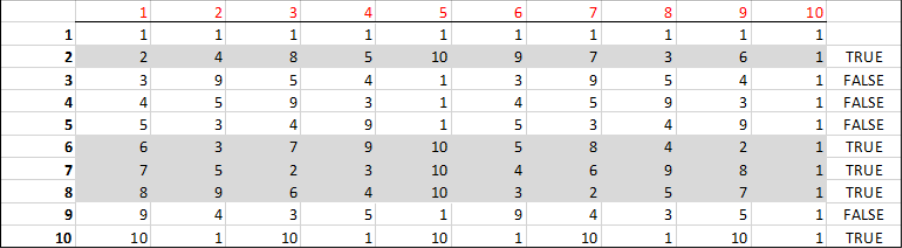
\includegraphics[width=0.8\textwidth]{Assignment0x04/image/generators}
\end{figure}

ExcelFormula = MOD((“linke Spalte”\^”Obere Zeile”);11)

The marked lines (2, 6, 7, 8) are generators.

\subsection{Calculate 42\textsuperscript{497} in Z\textsubscript{1361} using fast exponentiation and a handheld calculator (not the one running on your computer or a programming language). Document a, e and n for each step.
}

Fastexp(a=42, n=497)\\
1st Iteration:\\

e = 1\\
n is odd:\\
e = (42 * 1) mod 1361 = 42\\
a = 42² mod 1361 = 1764 mod 1361 = 403\\
n = 497 / 2 = 248\\

2):\\     

e = 42\\
n is even:\\
a = 403² mod 1361 = 450\\
n = n/2 = 124\\

3)\\

e = 42\\
n is even:\\
a = 450² mod 1361 = 1072\\
n = 124 / 2 = 62\\

4)\\

e = 42\\
n is even:\\
a = 1072² mod 1361 = 500\\ 
n = 62 /2 = 31\\

5)\\

e = 42\\
n is odd:\\
e = (500 * 42) mod 1361 = 585\\
a = 500² mod 1361 = 937\\
n = 31 / 2 = 15\\

6)

e = 1072\\
n is odd:\\
e = (937 * 585) mod 1361 = 1023\\
a = 937² mod 1361 = 124\\
n = 15 / 2 = 7\\

7)\\

e = 46\\
n is odd:\\
e = (124 * 1023) mod 1361 = 279\\
a = 124² mod 1361 = 405\\
n = 7 / 2 = 3\\

8)\\

e = 260\\
n is odd:\\
e = (405*279) mod 1361 = 32\\
a = 405² mod 1361 = 705\\
n = 3 / 2 = 1\\

9)\\

e = 503\\
n is odd:\\
e = (705*32) mod 1361 = 784\\
a = 705² mod 1361 = 260\\
n = 1 / 2 = 0\\

10)\\

$n = 0 =>$ return e = 784\\

$=> 42497$ mod 1361 = 784







